% ===================================================================================================
%                                                 |                                                 |
%                                                 |                                                 |
% -------------------------------------------- SECTION ---------------------------------------------|
%                                                 |                                                 |
%                                                 |                                                 |
% ===================================================================================================
\section{Use case: Smart factory}\label{sec_use_case}
% ---
%\begin{figure*}[!h]
%	\centering
%	\hspace*{\fill}
%	\subfloat[]{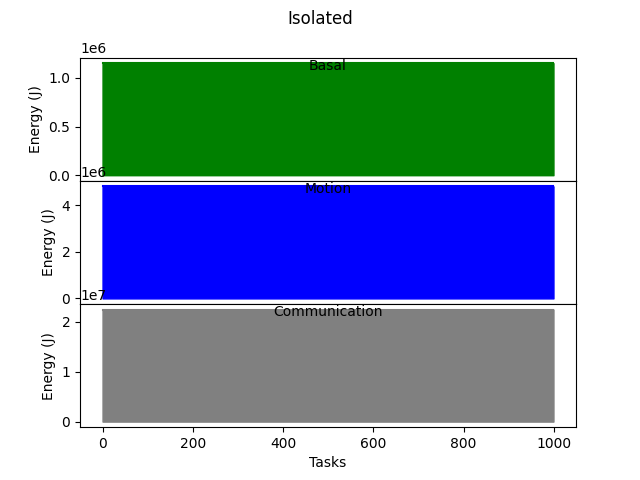
\includegraphics[width= 0.90\columnwidth]{fig/isolated_corrected.png} \label{fig:iso_energy}}
%	\hfill
%	\subfloat[]{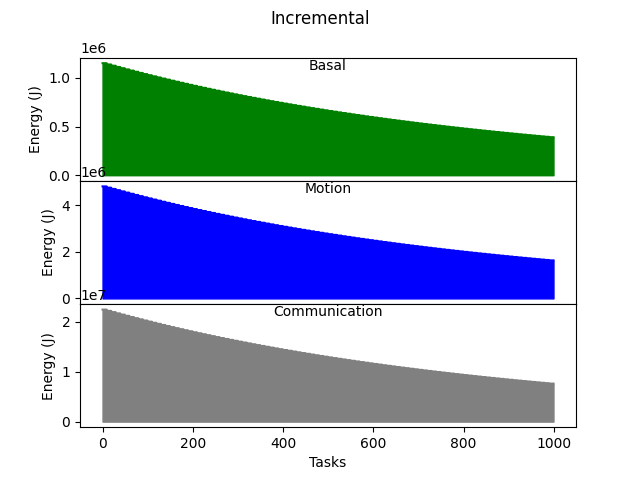
\includegraphics[width= 0.90\columnwidth]{fig/incremental_corrected.png} \label{fig:itl_energy}}
%	\hspace*{\fill}
%	\\%[-2ex]
%	\hspace*{\fill}
%	\subfloat[]{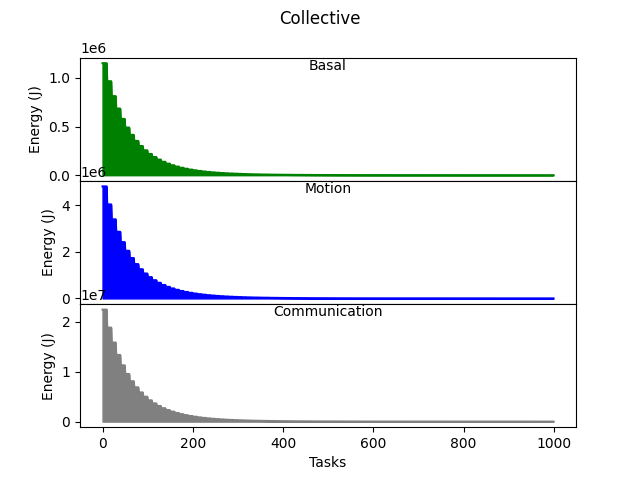
\includegraphics[width= 0.9\columnwidth]{fig/collective_corrected.png}\label{fig:cl_energy}}
%	\hfill    
%	\subfloat[]{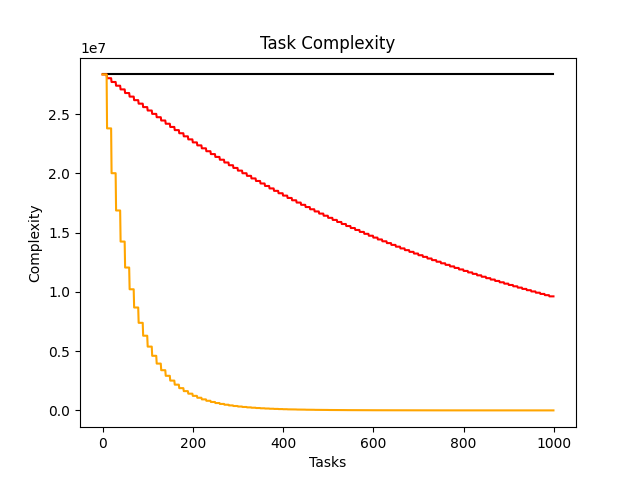
\includegraphics[width= 0.9\columnwidth]{fig/task_complexity.png}\label{fig:use_case_complexity}}
%	\hspace*{\fill}    
%	\caption[] {\label{fig:use_case_results} Energy expenditure per task: \subref{fig:iso_energy} isolated learning, \subref{fig:itl_energy} incremental+transfer learning,  \subref{fig:cl_energy} collective learning. \subref{fig:use_case_complexity} Scaling of the task complexity.}
%\end{figure*}
% ---
The goal of this section is to forecast the energy demand that EAI agents following the learning paradigms discussed in Sec.~\ref{sec:learning_paradigms} would have in a prototypical instance of a hypothetical smart factory. In this mock factory a pool $\mathcal{S}$ of $N_\mathcal{S}= 512$ industry relevant skills is divided into $N_\mathcal{K}=4$ clusters of $N_\mathcal{Z} = 128$ skills each. Additionally, consider that $m=32$ robots are available to learn the skills and that a skill is considered learned once the remaining knowledge goes below $\epsilon = 0.01$. For all the skills, the fundamental skill complexity is $c_0 = 100$ episodes.
% whose purpose is to execute a series of tasks, drawn from a pool $ \mathcal{T} $ of . In the example we consider \hl{a set of $N_{\mathcal{T}}=1,000$ related and similar tasks}; that is $ \mathcal{T}=\left\lbrace \tau_1,\ldots, \tau_{1000} \right\rbrace$, where we assume $ \tau_i \sim \tau_j $. These tasks will need to be learned by an embodied AI agent so that they can be executed and used in production. We will explore what would be the consequences of the isolated (what we call inefficient) learning paradigm and the envisioned, and arguably desired, collective learning paradigm. 

The power in \eqref{eq:energy_per_episode} is composed by the sum of the power required for basal processes, the power for motion and interaction, and the power for computation and communication; i.e.
% ---
\begin{equation}
    P_0 = P_{BEE}+P_{MIE} + P_{CCE}.
\end{equation}
% ---
To choose $P_{BEE}$, we consider that the smart factory will be populated with state-of-the-art tactile robots, like the Franka Emika Robot, which requires a typical power of about $\unit[72]{W}$. To approximate $P_{MIE}$, we use the fact that, in demanding tasks, the power demand of the system can go up to a maximum of about $ \unit[300] {W} $. Finally, to determine $P_{CCE}$, we make the assumption that, to deal with the computing effort that learning new skills will have on the robots' local processors, the smart factory will delegate the computational burden to a remote computing unit (i.e. cloud computing). Thus, we take as reference the work in \cite{Strubell2019EnergyAP}, where a state-of-the-art machine learning algorithm executed in a cluster required $\unit[1,415.78]{W}$ to solve a task. Additionally, without loss of generality, we can assume that each trial episode takes $\Delta t = 60$ seconds to execute. Using these reference values, we can estimate that, when learning a skill, a trial episode has en energetic demand of:
% ---
\begin{equation}
	e_0 = P_0 \Delta t = \left(70 + 300 + 1,415.78\right) \left(60\right) \approx 105~\text{kJ}
\end{equation}
% ---
Regarding the knowledge exchange efficiency constants, they are chosen as follows
% ---
% ---
\begin{itemize}
	\item $\alpha =  0.0461$ (in accordance to \eqref{eq:isolated_learning_rate})
	\item $\delta =  0.0360$ (see \eqref{eq:delta})
	\item $\eta= 0.1$
\end{itemize} 
% ---
%\begin{align}\label{eq:transfer_constants}¸
%\begin{split}
%    \alpha &=1\times10^{-3}\\
%    \beta &=1\times10^{-5}\\
%    \gamma &=1\times10^{-7}    
%\end{split}
%\end{align}
% ---
%Finally, we assume that each episode $n$ contains $k=10,000$ iterations.

% ===================================================================================================

%\subsection{Summary}
%
%The equation for incremental learning is equivalent to \eqref{eq:knowledge_exponential_form} with $r=1$ since no inter-agent exchange of knowledge occurs and $\beta_k = 0$,¸ as knowledge from other cluster cannot be used.
% ---
%\begin{figure*}[!th]
%	\centering
%	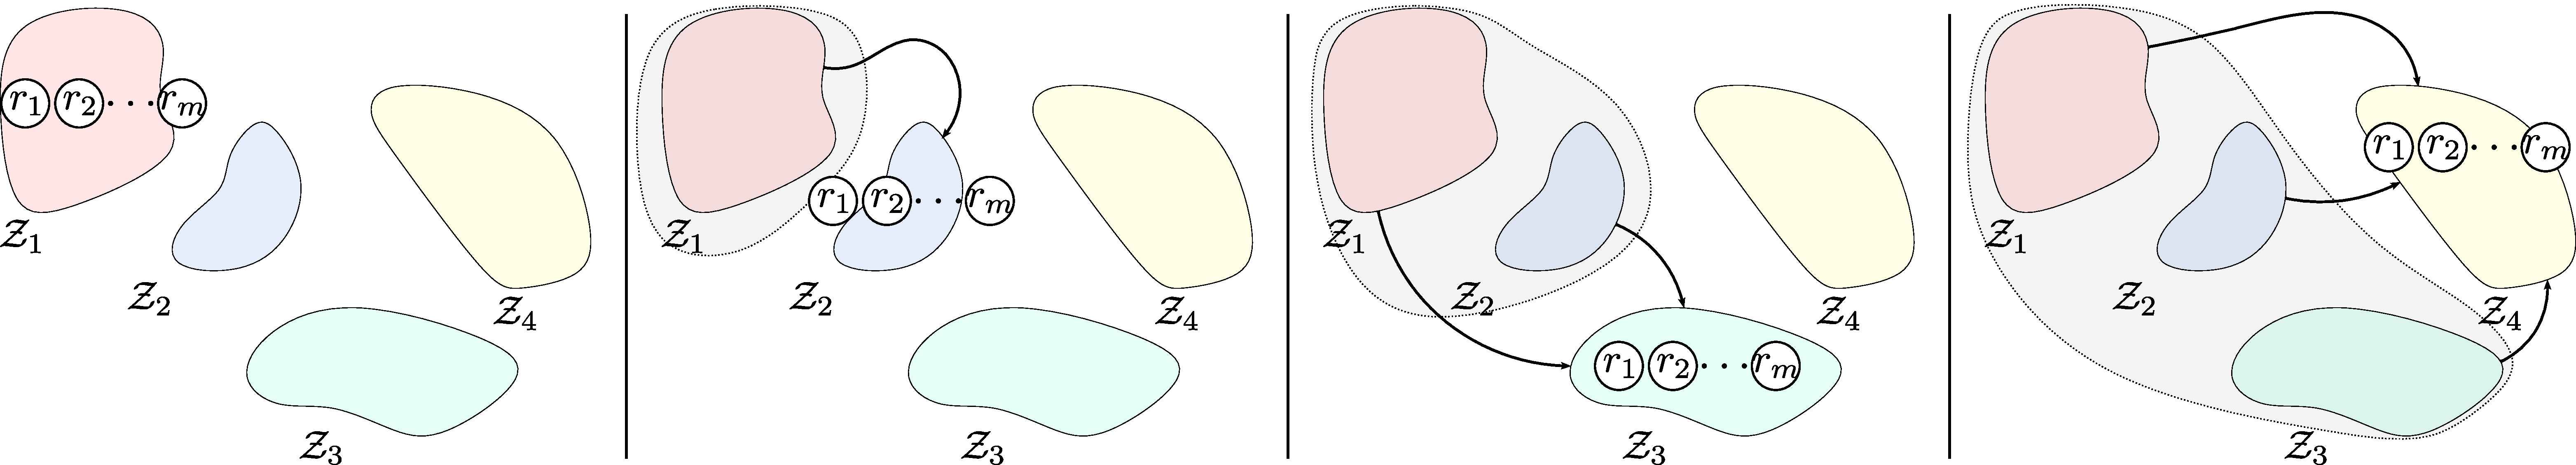
\includegraphics[width=0.95\textwidth]{fig/cluster_learning_sequence.pdf}
%	\caption{The sequence followed to learn the clusters.}
%	\label{fig:cluster_learning_sequence}
%\end{figure*}
% ---
%---


%\begin{figure*}[!t]
%	\centering
%	\hspace*{\fill}
%	\subfloat[]{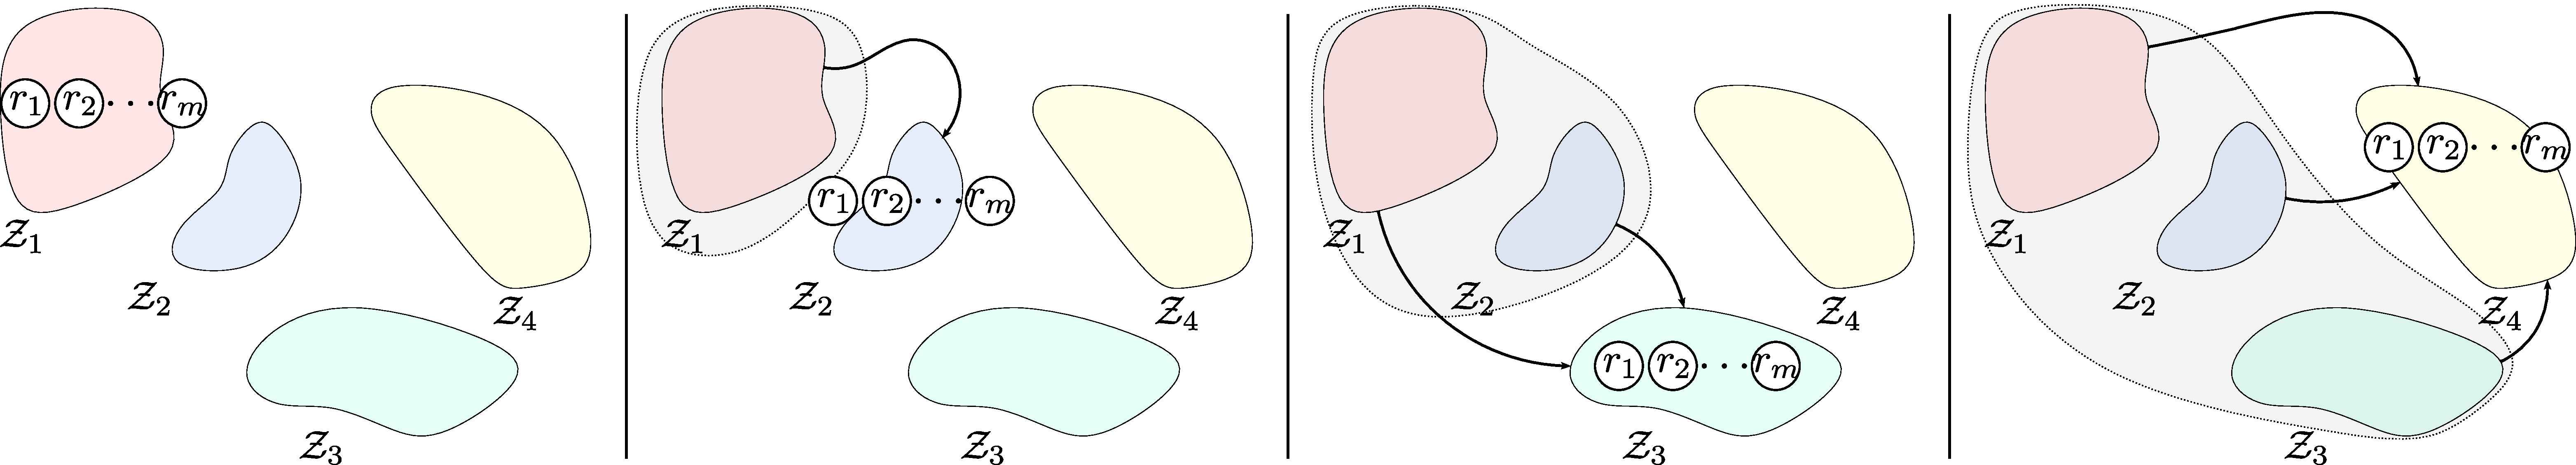
\includegraphics[width= 0.8\textwidth]{fig/cluster_learning_sequence.pdf} \label{fig:cluster_learning_sequence}}
%	\hspace*{\fill}
%	\\	
%	\hspace*{\fill}
%	\subfloat[]{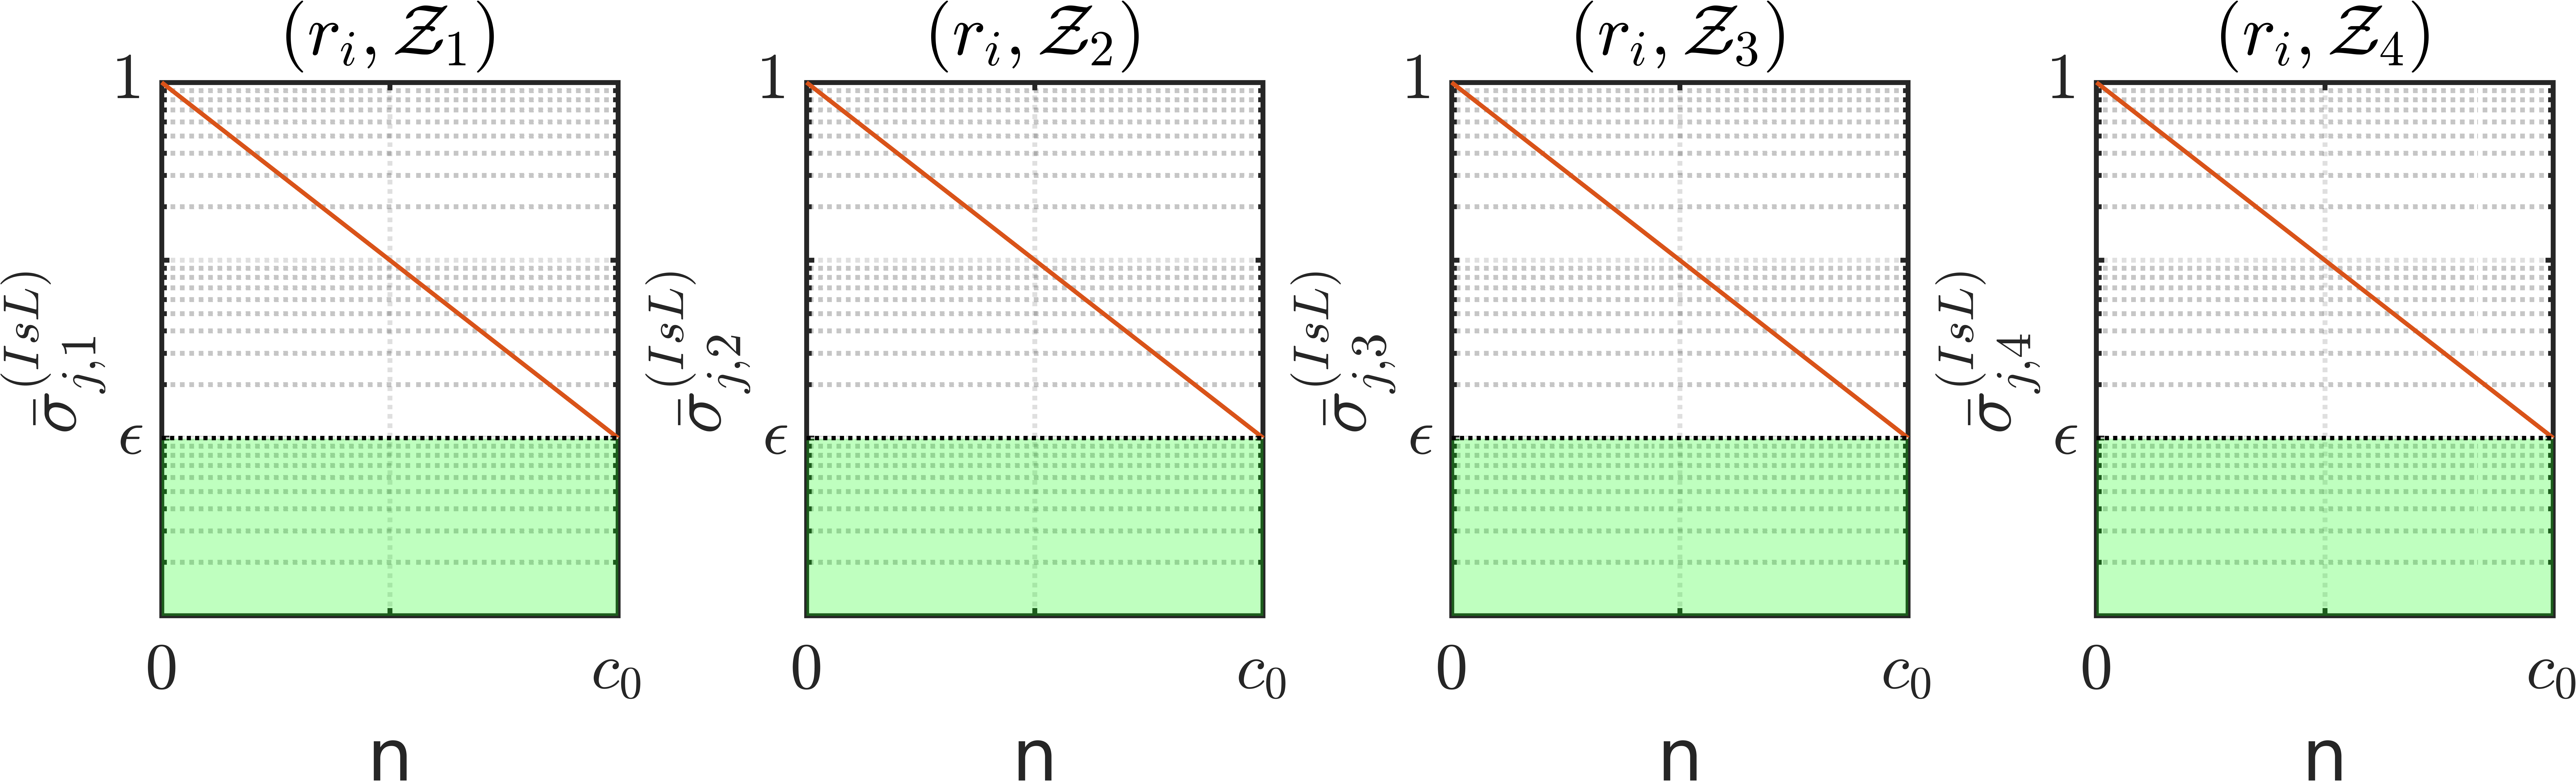
\includegraphics[width= 0.8\textwidth]{fig/dynamics_isolated_learning.pdf} \label{fig:dynamics_isolated_learning}}  
%	\hspace*{\fill}
%	\\	
%	\hspace*{\fill}
%	\subfloat[]{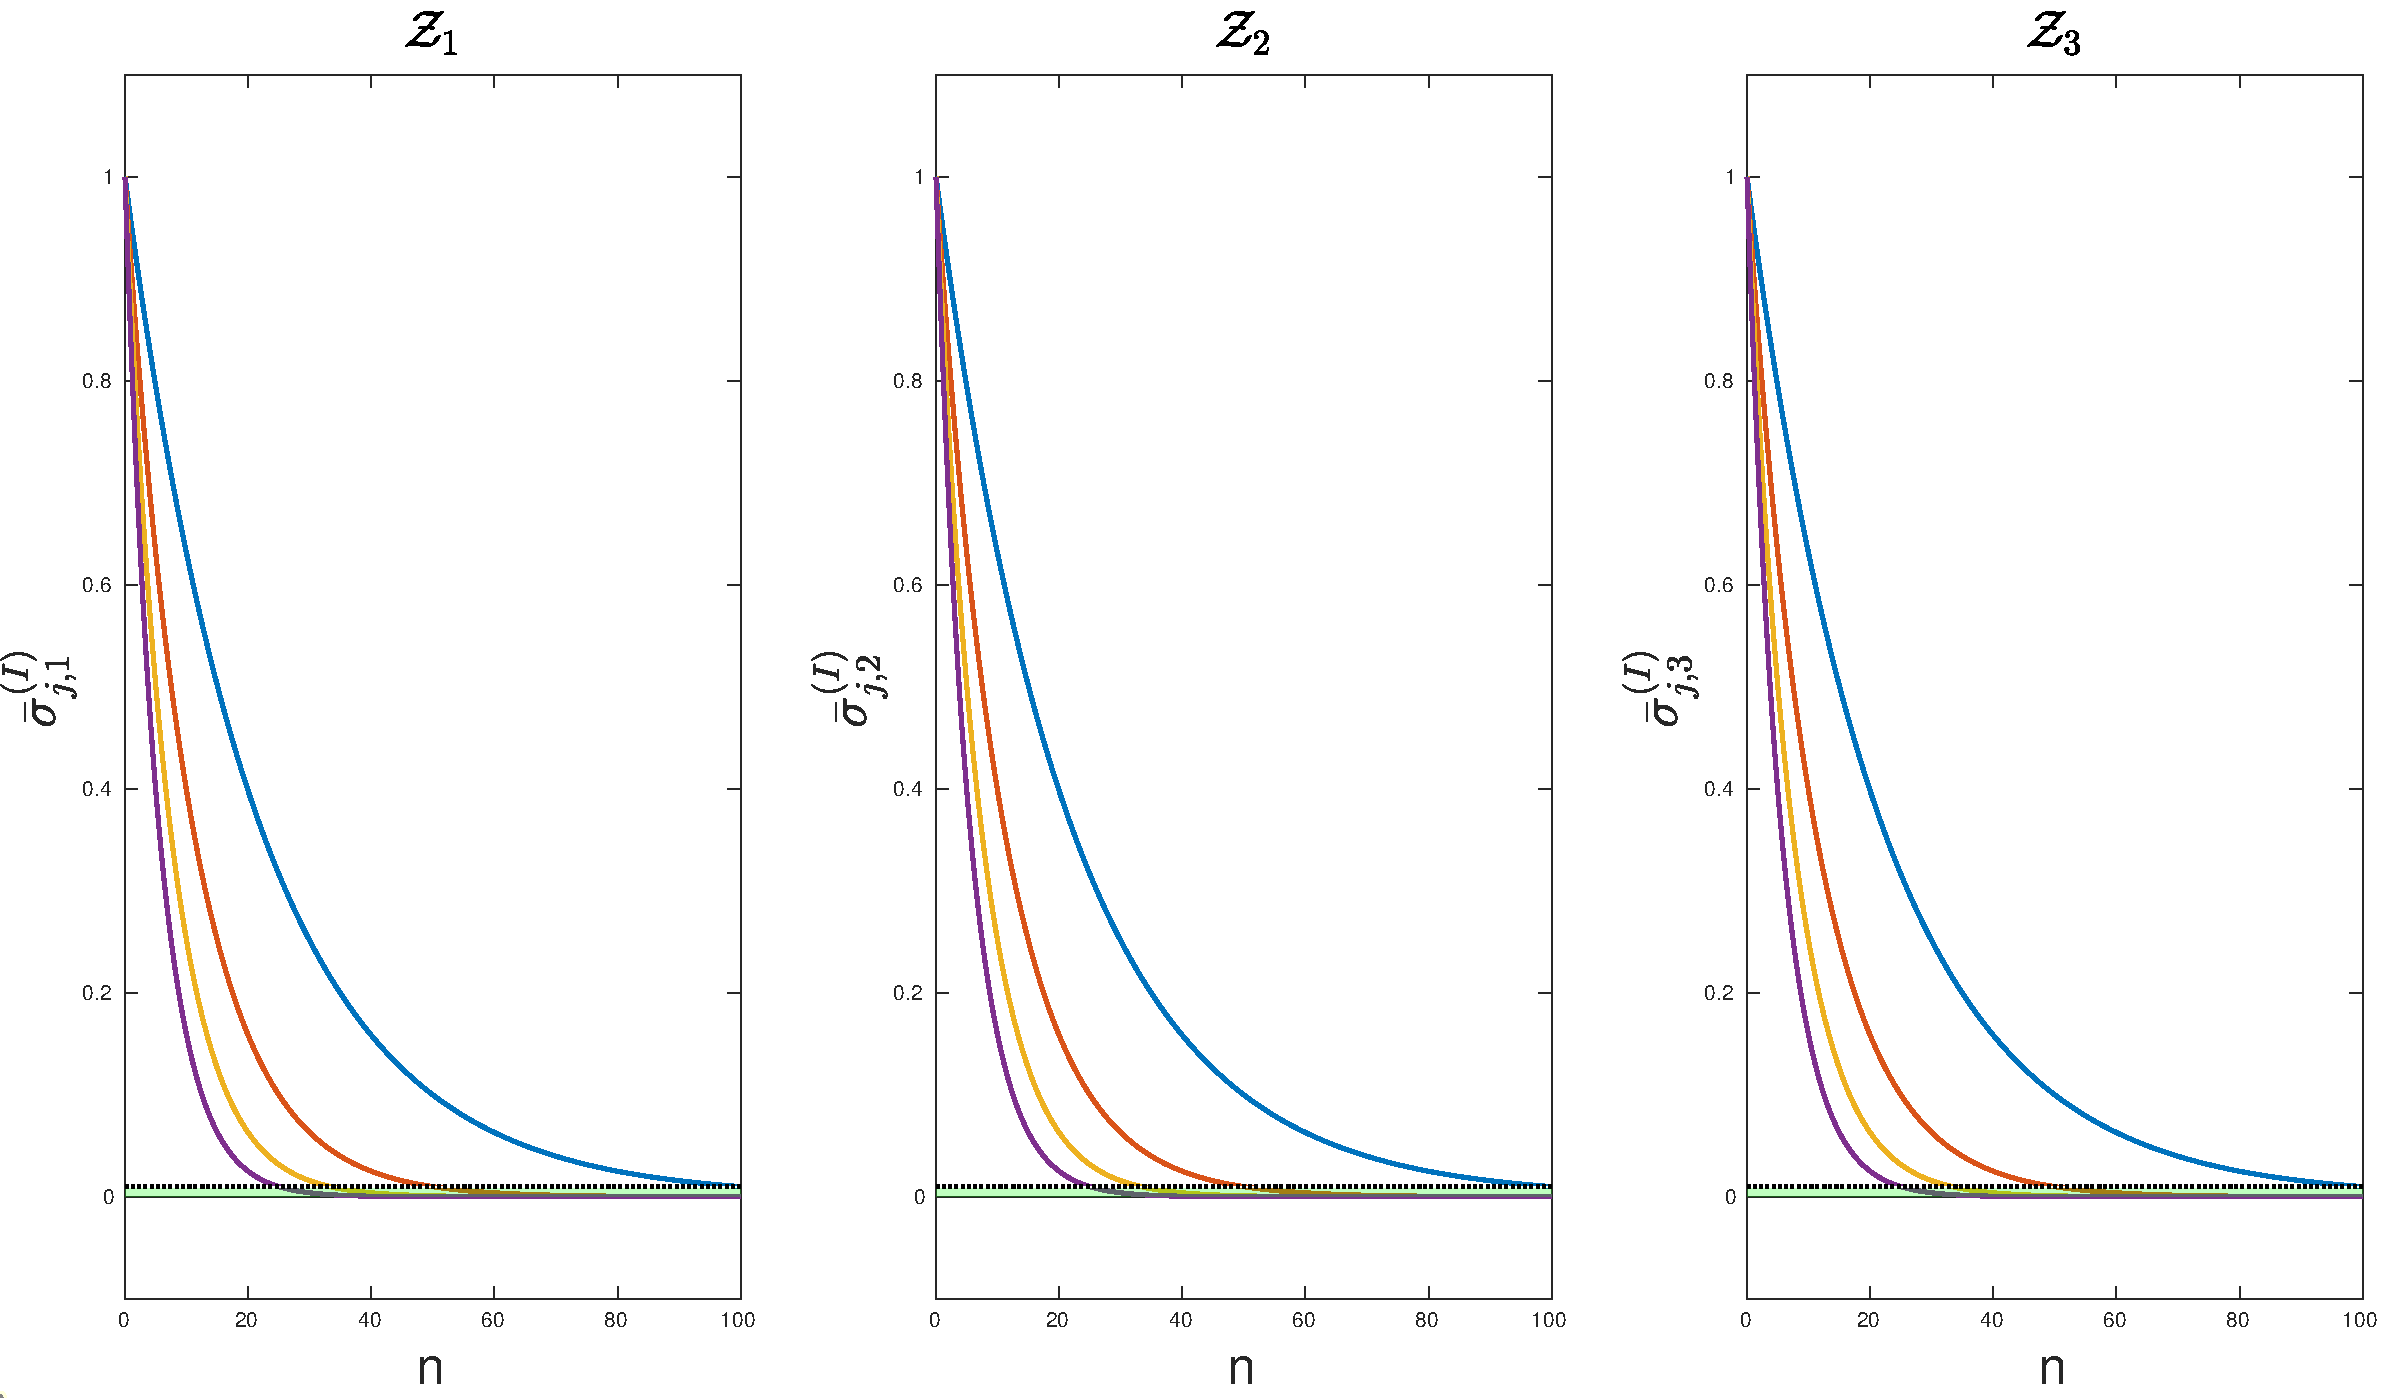
\includegraphics[width= 0.8\textwidth]{fig/dynamics_incremental_learning.pdf} \label{fig:dynamics_incremental_learning}}  
%	\hspace*{\fill}	
%	\\
%	\hspace*{\fill}
%	\subfloat[]{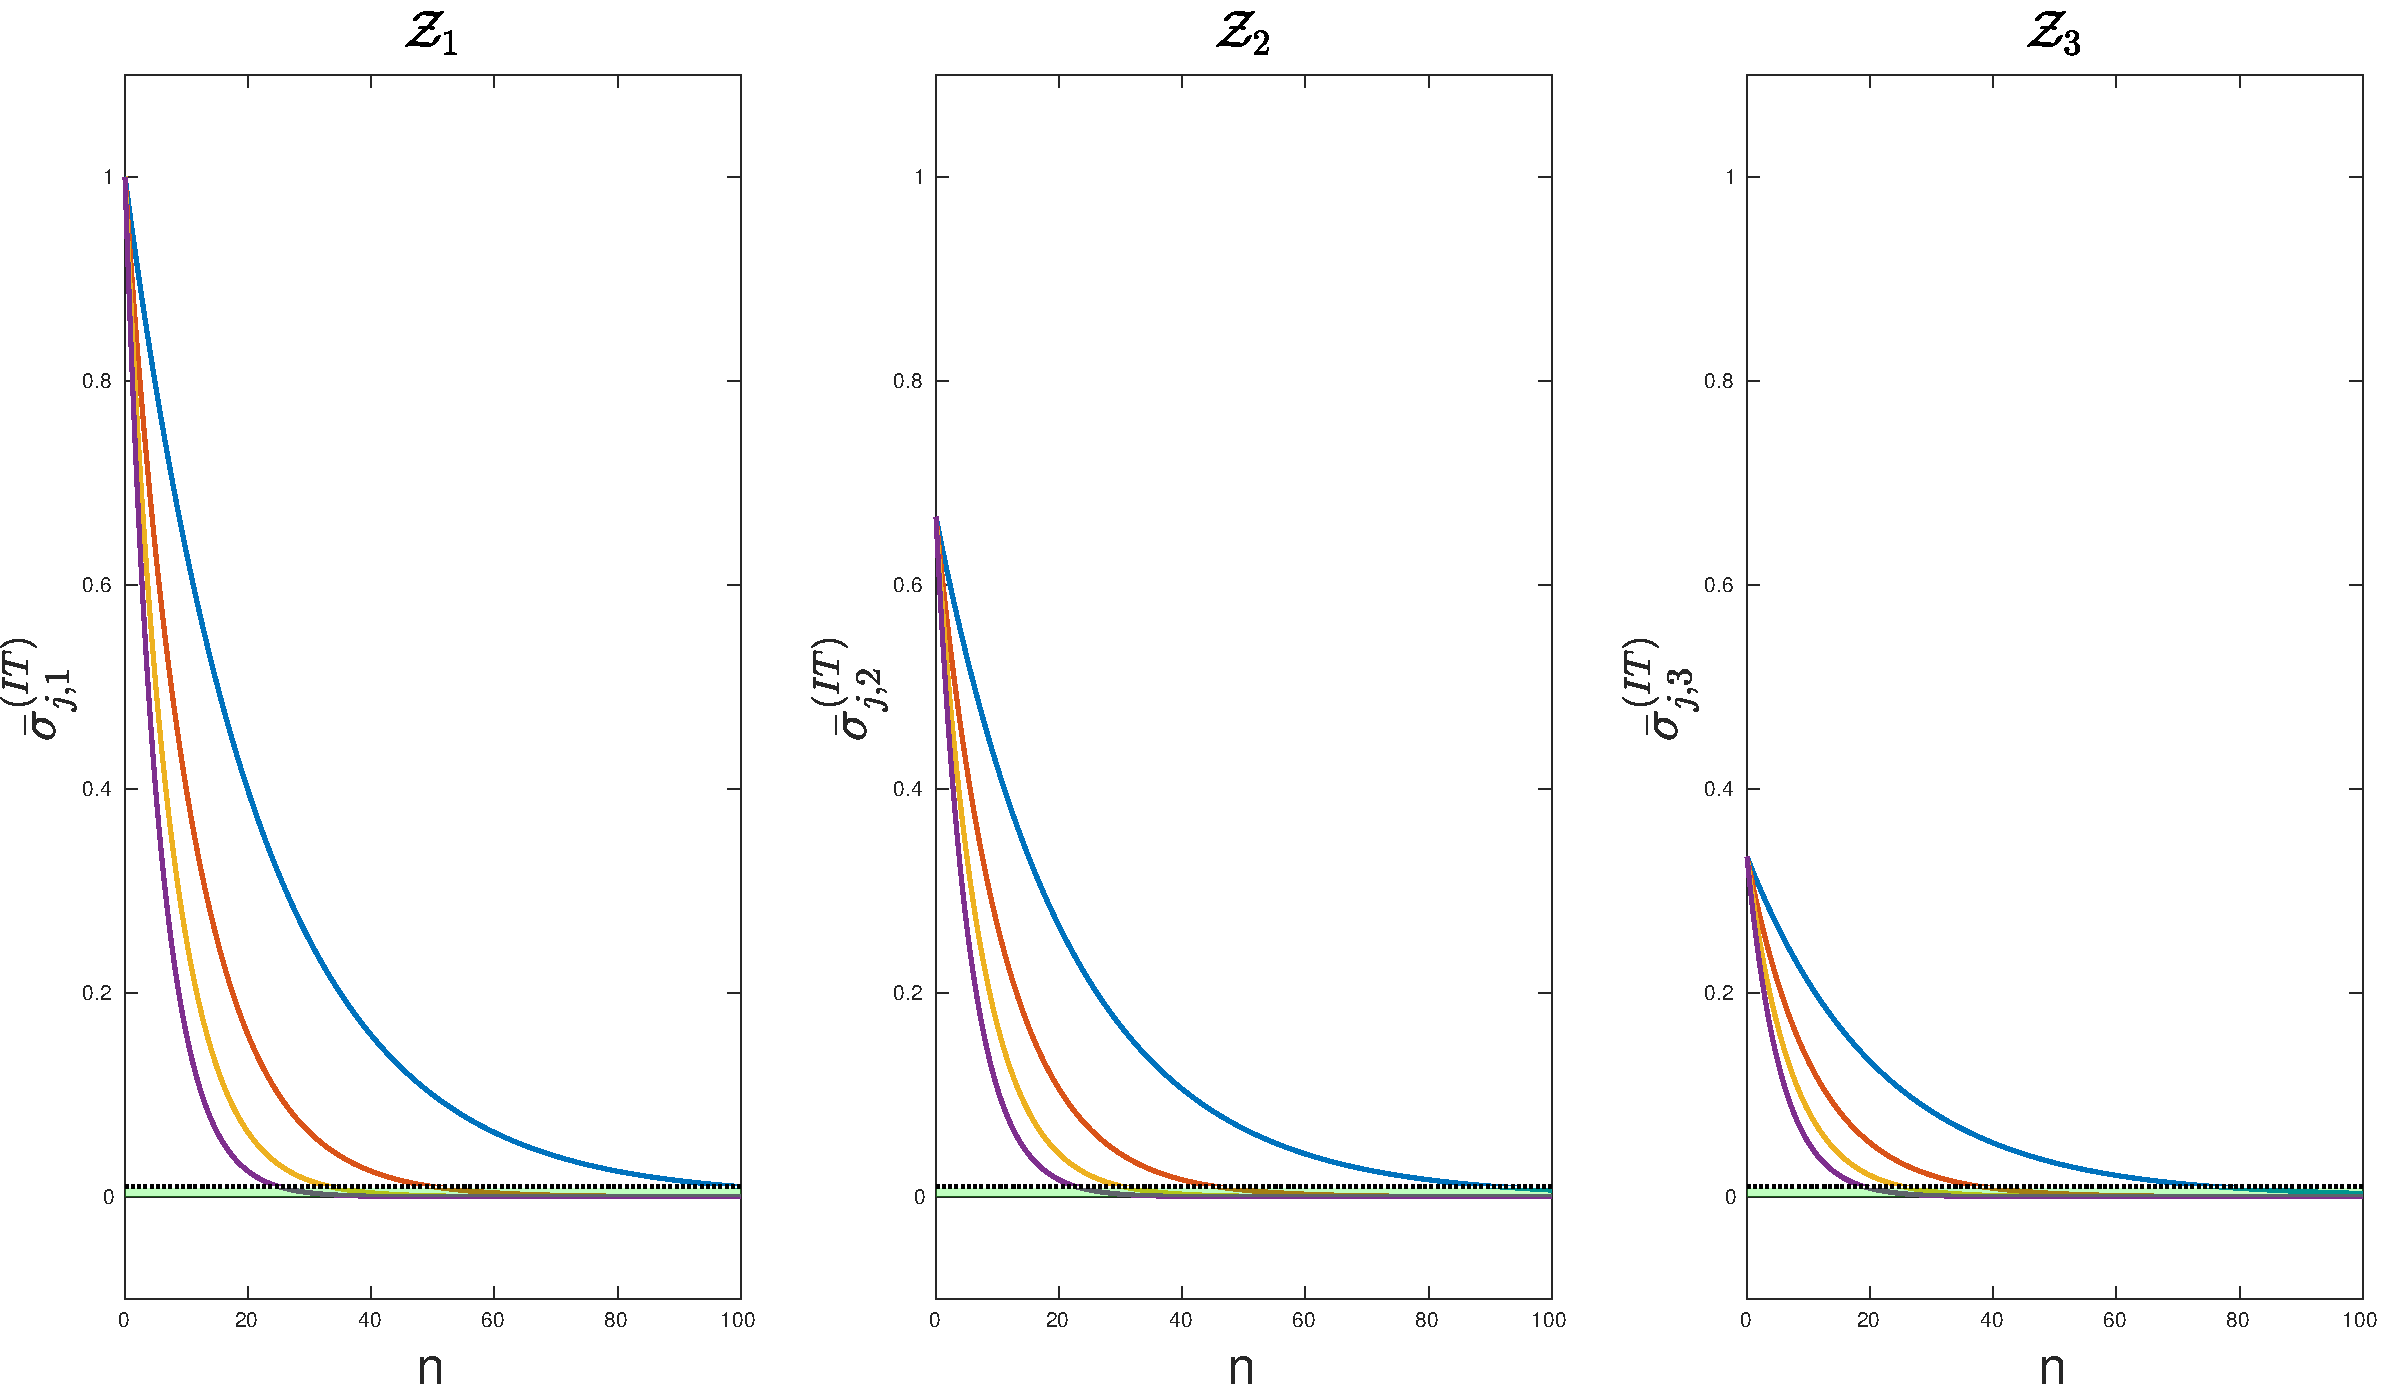
\includegraphics[width= 0.8\textwidth]{fig/dynamics_incremental_transfer_learning.pdf} \label{fig:dynamics_incremental_transfer_learning}}  
%	\hspace*{\fill}
%	\\
%	\hspace*{\fill}
%	\subfloat[]{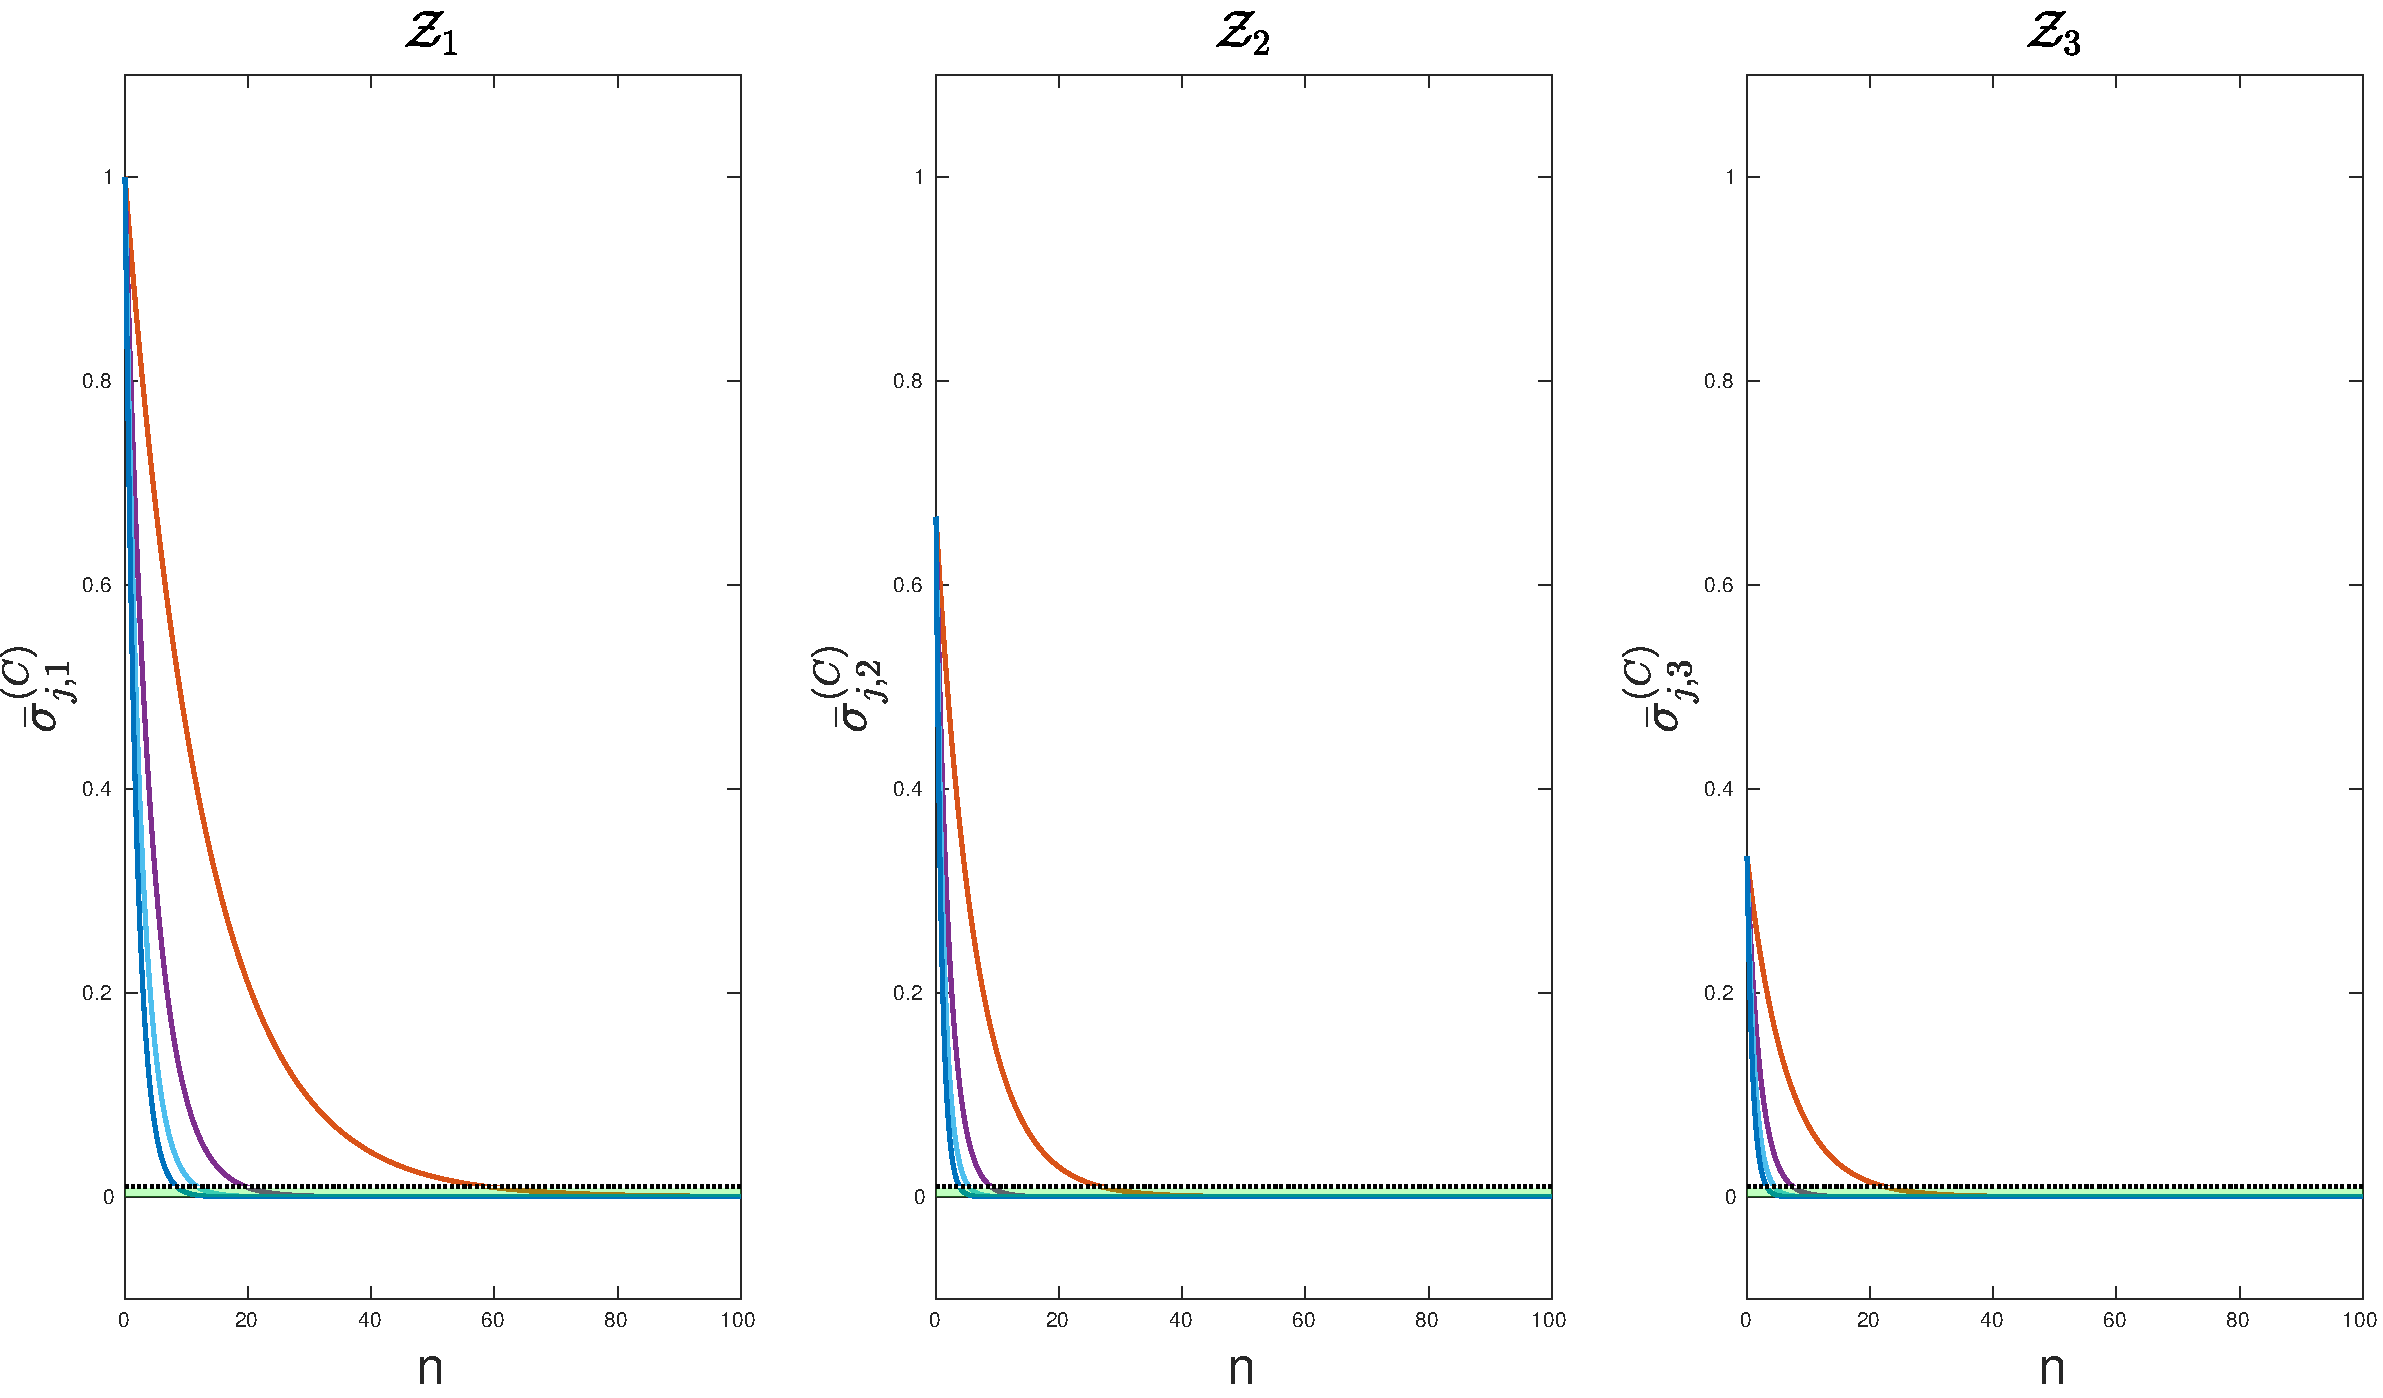
\includegraphics[width= 0.8\textwidth]{fig/dynamics_collective_learning.pdf} \label{fig:dynamics_collective_learning}}
%	\hspace*{\fill}
%	\caption[] {\label{fig:collective_learning} Scenario 1: \subref{fig:cluster_learning_sequence} the skills of each cluster are learned by the $ m$ robots in succession, \subref{fig:dynamics_isolated_learning} isolated learning,  \subref{fig:dynamics_incremental_learning} incremental learning,  \subref{fig:dynamics_incremental_transfer_learning} incremental + transfer learning, \subref{fig:dynamics_collective_learning} collective learning.}
%\end{figure*}
% ---

% ===================================================================================================
\subsection{The skill complexity of the different paradigms}
The remaining knowledge for the four skills learned per robot are shown in Fig.~\ref{fig:collective_learning} in logarithmic scale. With the parameters discussed previously the $m$ robots are used to learn in parallel the $N_\mathcal{Z}$ skills of each cluster in succession, as shown in Fig.~\ref{fig:cluster_learning_sequence}. Notice that as expected, isolated learning (Fig.~\ref{fig:dynamics_isolated_learning}) exhibits the worst performance, always requiring $c_0$ episodes to learn every single skill. Since incremental learning (Fig.~\ref{fig:dynamics_incremental_learning}) does not benefit from the knowledge from the previously visited clusters, a robot $r_i$ needs to start accumulating knowledge from the beginning every time it moves to a different cluster. This is not the case in transfer learning (Fig.~\ref{fig:dynamics_incremental_transfer_learning}), as the more clusters a robot has visited the faster a new skill is learned. The speed of knowledge collection is clearly exponentiated with collective learning (Fig.~\ref{fig:dynamics_collective_learning}) thanks to the exchange of knowledge among the $m$ robots. In comparison to the other learning paradigms, with CL the skills are learned within a few trial episodes in every cluster. 

To assess how the number $m$ of robots affects the total number of trial episodes $C_\mathcal{S}$ required to learn all the $N_\mathcal{S}$ skills we use the same parameters as before but vary $m \in \left \lbrace 2,4,8,16,32,64,128\right \rbrace$. Moreover, we considered an additional collective learning scenario in which, unlike the previous case, the total number of available robots is distributed equally among the clusters to benefit from transfer learning at an earlier time during learning. The results are shown in Fig.~\ref{fig:total_episodes_per_n_robots}. From it, it can be seen that, at first, incremental learning is better than the trivial isolated learning case; however, as the number or robots increases, the skill knowledge is divided among the available robots which implies that less knowledge can be passed, as the pool of learned sills $\zeta_k$ per robot gets smaller. This explains why the total number of trial episodes for IsL and IL approach each other in the limit. TIL exhibits a similar behavior, as the number of robots grows, less cluster knowledge can be collected by each robot and transferred to the next cluster. Indeed, TIL rapidly converges to IL and eventually to IsL. In CL, a similar effect shows that when all robots are learning skills in from the same clusters, as the number of robots grows, the total complexity approaches that of the same number of robots distributed across clusters.
% ---
%\begin{figure}[!th]
%	\centering
%	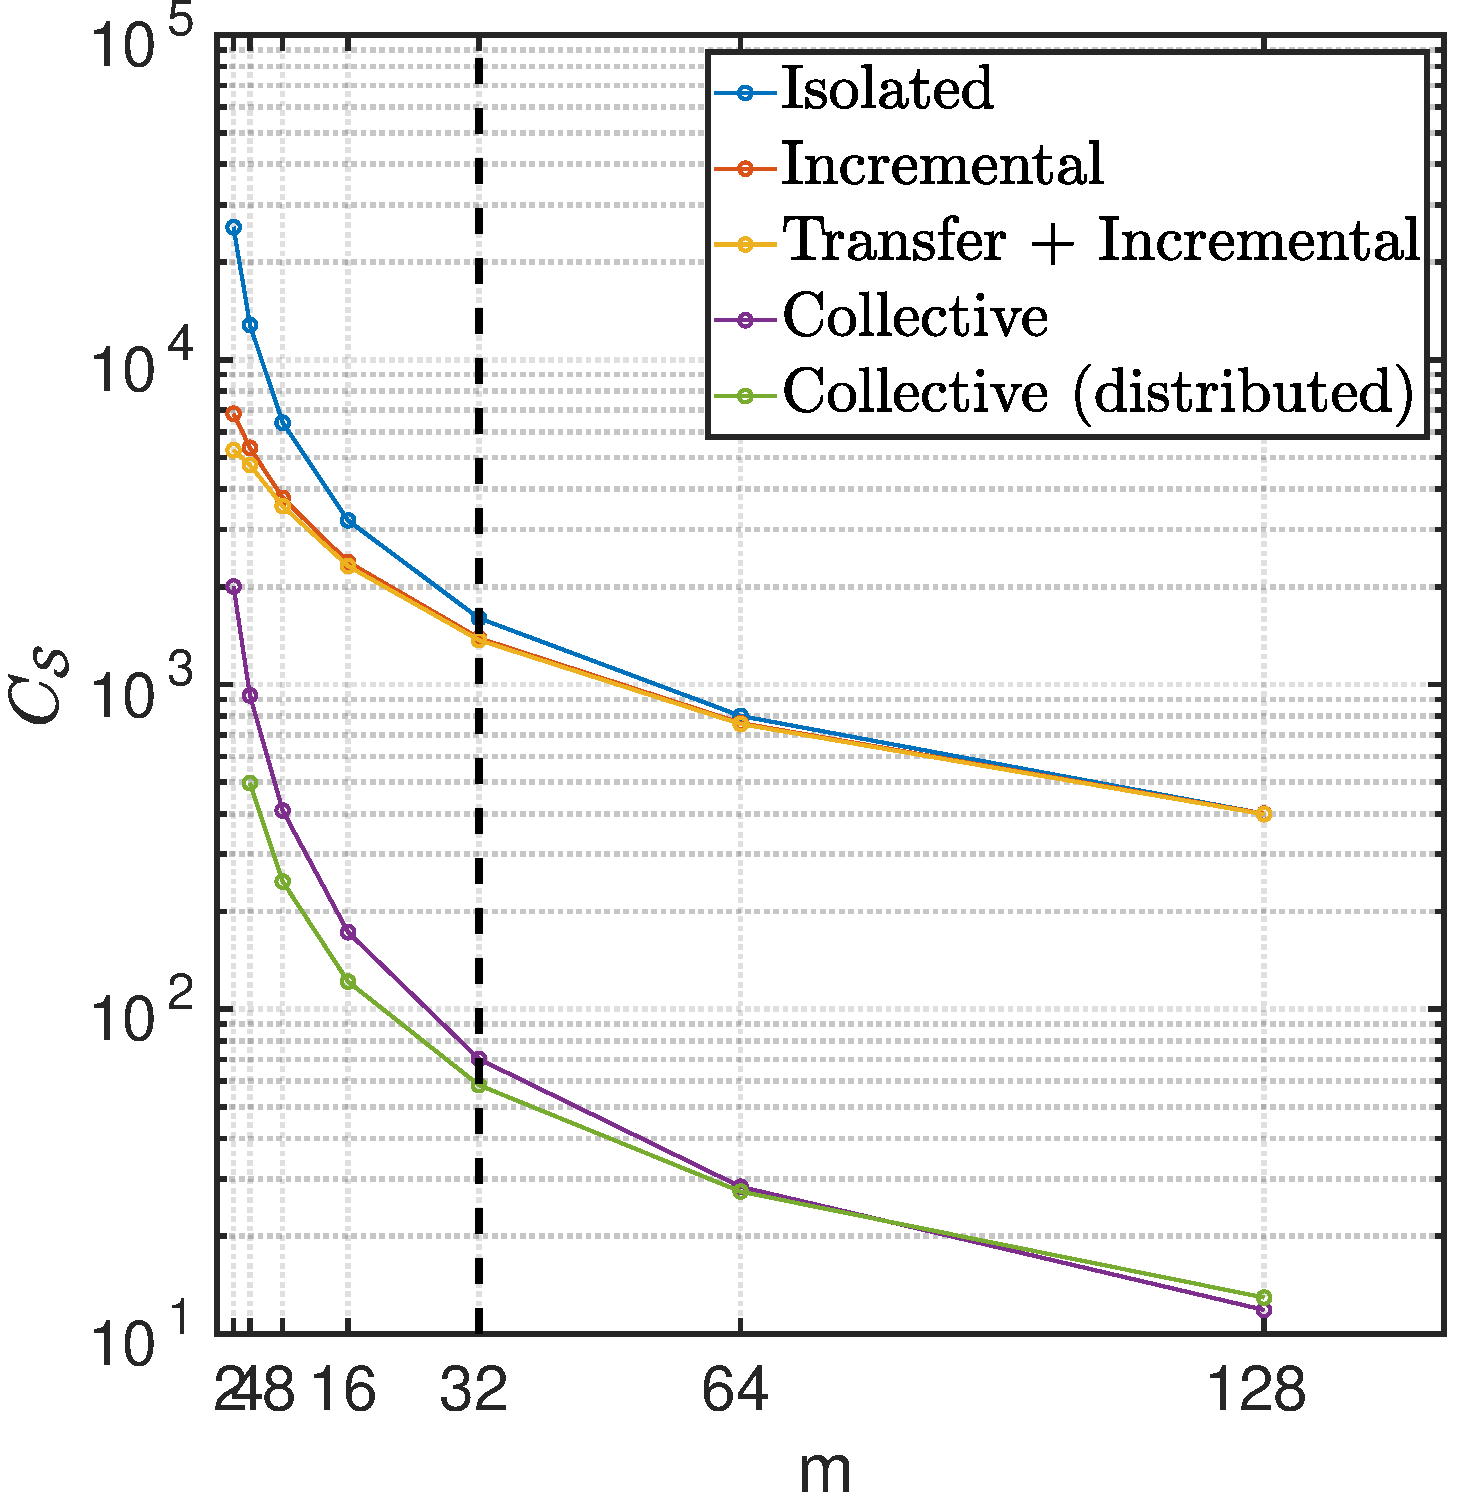
\includegraphics[width=0.9\columnwidth]{fig/total_episodes_per_n_robots.pdf}
%	\caption{Total number of episodes to learn the universe of skills as a function of the available robots.}
%	\label{fig:total_episodes_per_n_robots}
%\end{figure}
%% ---


% SUBSECTION ========================================================================================
\subsection{Energy consumption}
Consider that the results in Fig.~\ref{fig:total_episodes_per_n_robots} shows the total number of episodes required by each of the $m$ robots. To compute the total energy demand those numbers need to be scaled by the factor $m e_0$, which leads to the consumption shown in Fig.~\ref{fig:total_energy_per_n_robots}.
% ---
%\begin{figure}[!th]
%	\centering
%	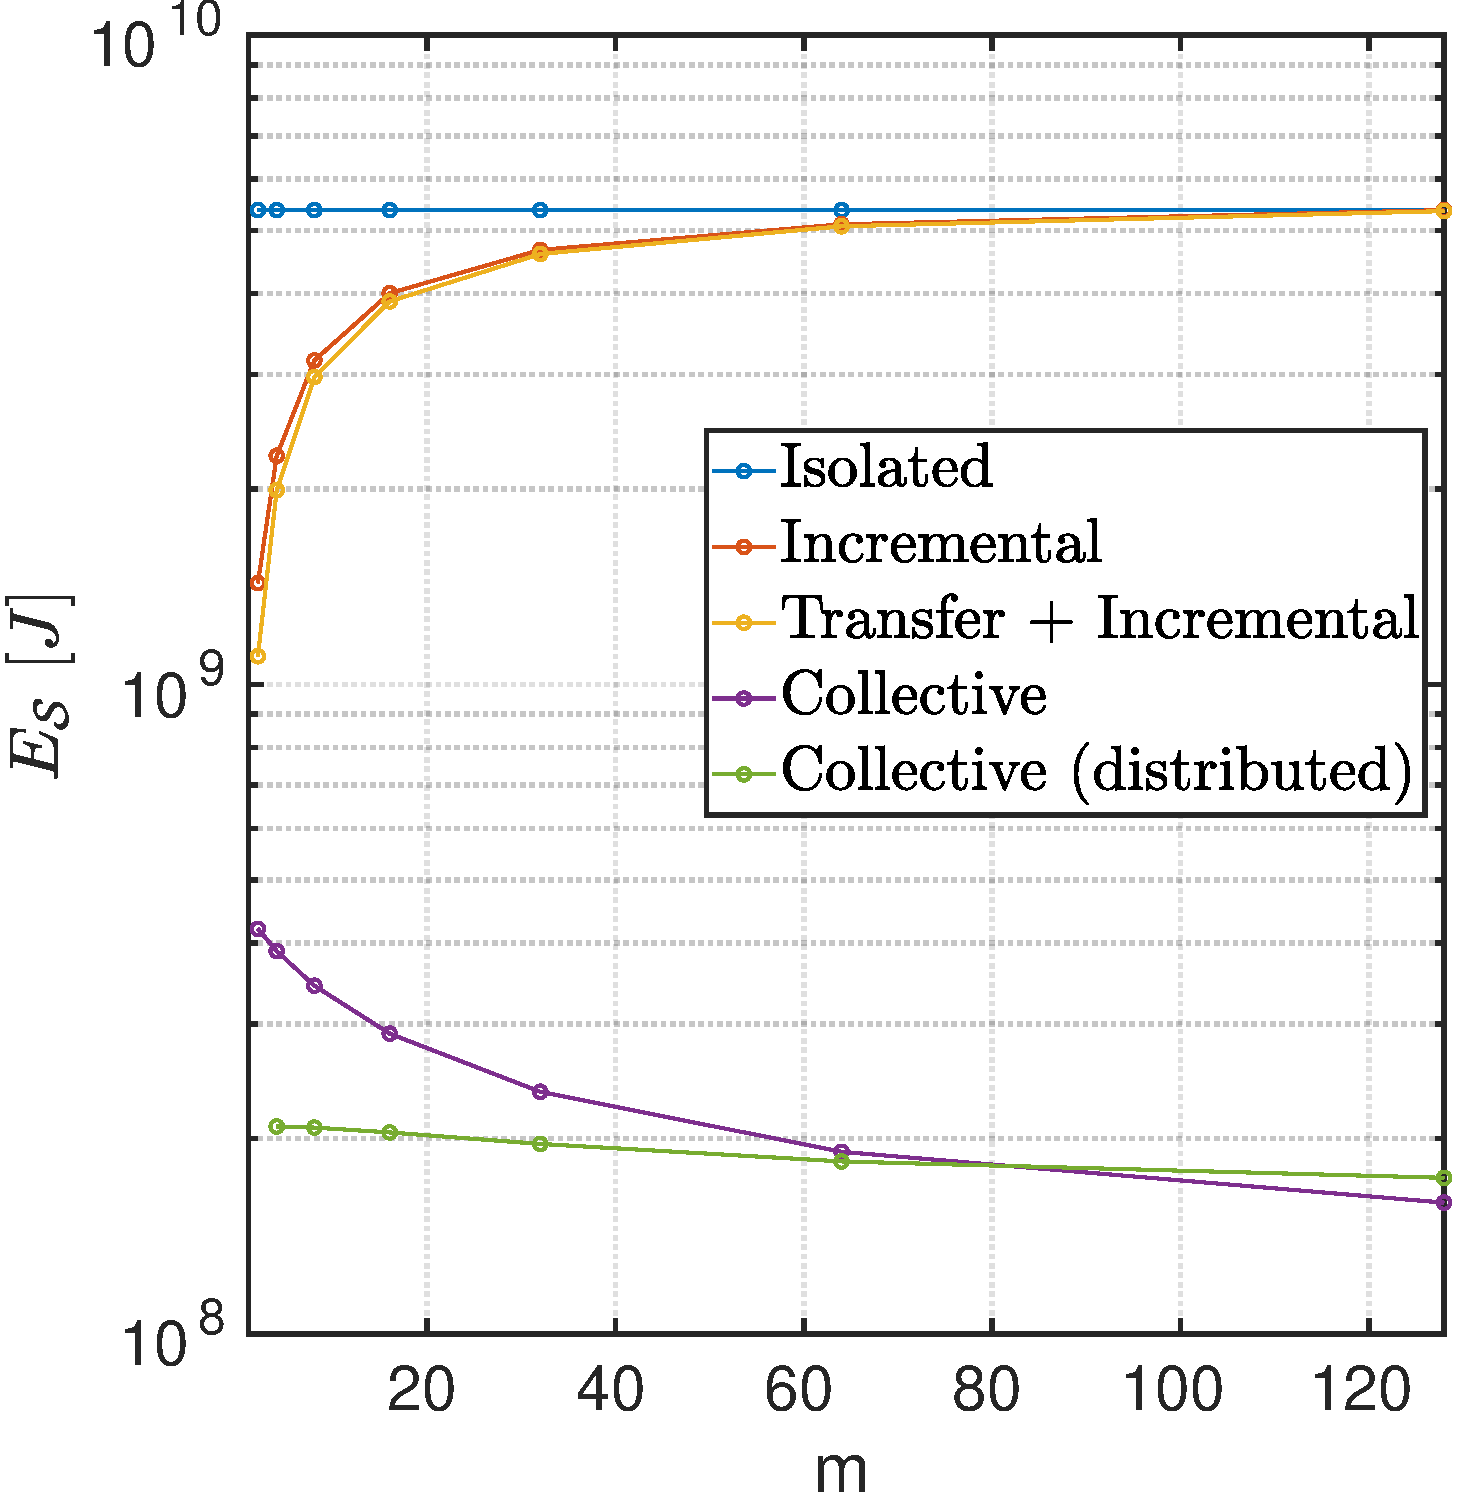
\includegraphics[width=0.9\columnwidth]{fig/total_energy_per_n_robots.pdf}
%	\caption{Total energy consumption.}
%	\label{fig:total_energy_per_n_robots}
%\end{figure}
%% ---

\begin{figure*}[!t]
	\centering
	\hspace*{\fill}
	\subfloat[]{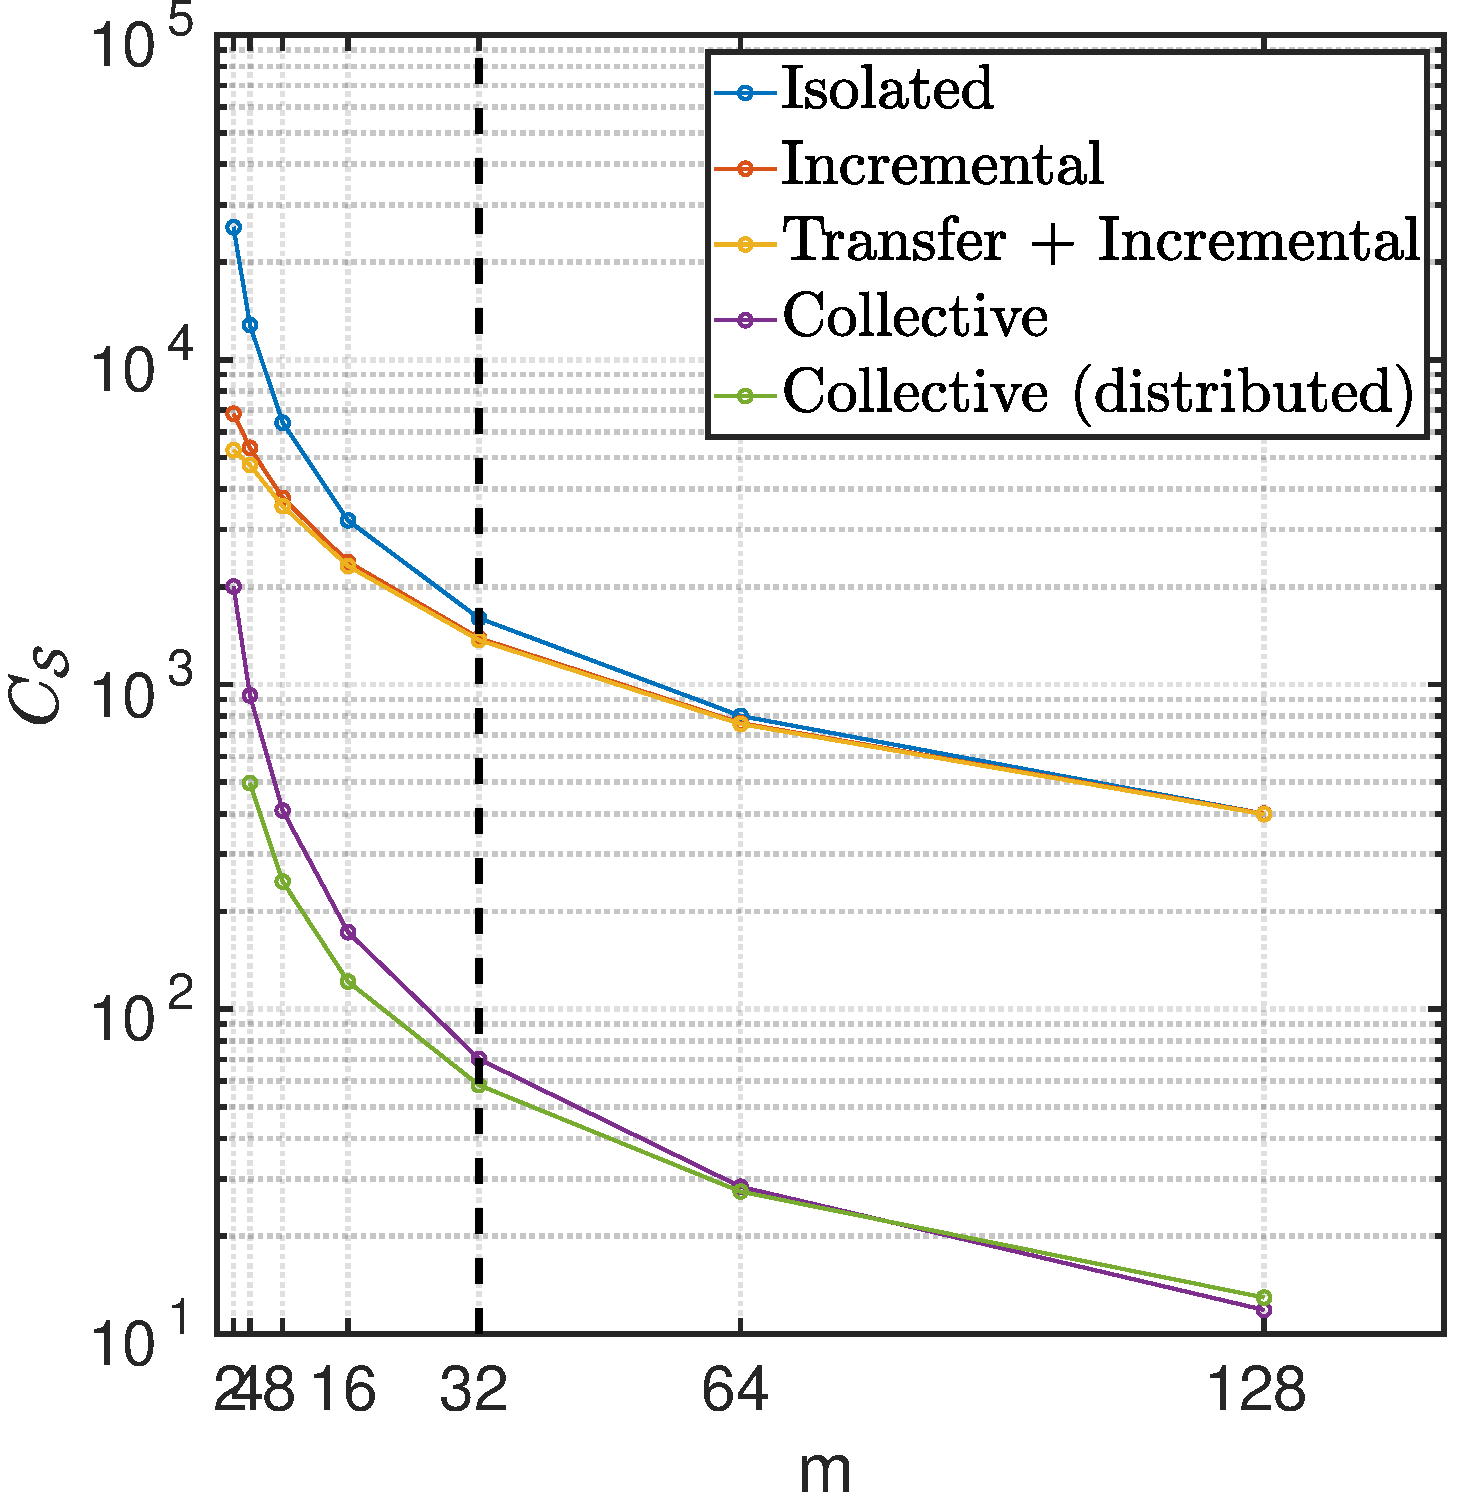
\includegraphics[width=0.45\textwidth]{fig/total_episodes_per_n_robots.pdf}
	\label{fig:total_episodes_per_n_robots}}  
	\hfill	
	\hspace*{\fill}
	\subfloat[]{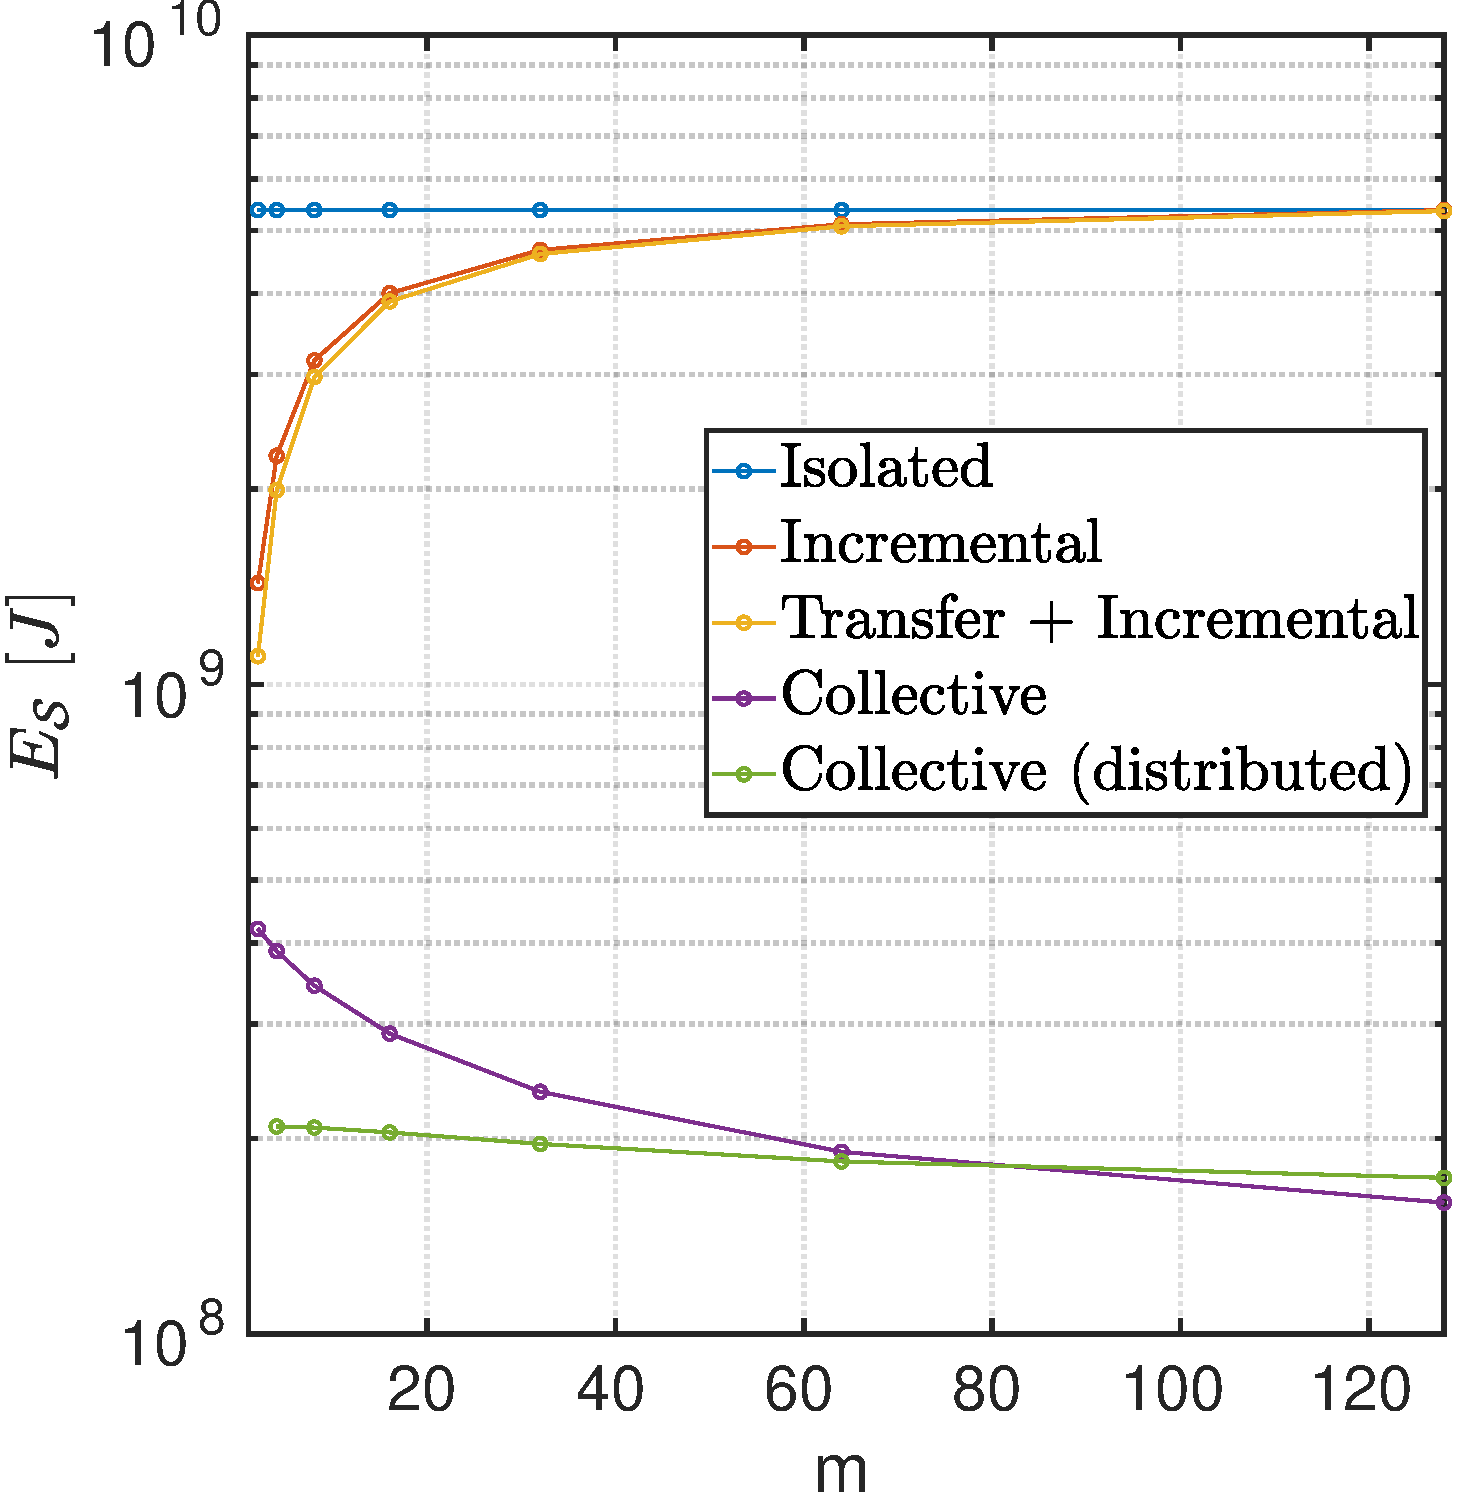
\includegraphics[width=0.45\textwidth]{fig/total_energy_per_n_robots.pdf}
	\label{fig:total_energy_per_n_robots}}
	\hspace*{\fill}
	\caption[] {\label{fig:final_results} The effect of the number of robots: \subref{fig:total_episodes_per_n_robots} Total number of episodes to learn the universe of skills as a function of the available robots and \subref{fig:total_energy_per_n_robots} the total energy consumption.}
\end{figure*}
% ---

Undoubtedly, collective learning shows that it has a not only the best energy usage of all the paradigms, but, inline the rest, the more robots are included the better energy usage. 

%Fig.~\ref{fig:iso_energy} shows the energy demand for a single task. Considering the parameters introduced above, we  estimate the energy and episodes needed by a single robot to learn all $N_{\mathcal{T}}$ tasks. For the episodes, we have
%% ---
%\begin{equation}¸
%    n^{Iso}_{\mathcal{T}} = N_{\mathcal{T}} \cdot c_j = 1,600\times 10 \times 100 = 1,600,000 \quad\text{episodes}.
%\end{equation}
%% ---
%With $P=\unit[1787.8]{W}$ and using \eqref{eq:energy_per_episode}-\eqref{eq:total_energy}. The total energy equates
%% ---
%\begin{equation}
%    E^{Iso}_{\mathcal{T}} = \unit[283.52]{GJ} %283,520,000,000.0,
%\end{equation}
%% % ---
% 
%% ---
%% SUBSECTION ========================================================================================
%\subsection{Incremental learning and transfer learning}
%%For ITL we consider a transfer factor of $\lambda=0.005$ to be used in \eqref{eq:similarity_metric}. Moreover, leveraging parallelization, $m=10$ robots learn $\frac{N_{\mathcal{T}}}{m} = 10$ tasks at the same time. 
%Then, using \eqref{eq:complexity_TIL}, \eqref{eq:itl_energy_per_task}, and \eqref{eq:itl_total_energy}; this results in the following episode and energy demands:
%% ---
%\begin{align}
%  n^{ITL}_{\mathcal{T}} &= 972,050\quad\text{episodes} \\
%  E^{ITL}_{\mathcal{T}} &= \unit[172.24]{GJ} % 172,247,385,965.70197
%\end{align}
%% ---
%% SUBSECTION ========================================================================================
%\subsection{Collective learning in the smart factory: a paradigm change}
%While incremental learning only takes the history of one robot into account, collective learning makes it able to use the already learned knowledge of all $m=10$ robots in the collective involved in the learning process. Using eqs. \eqref{eq:complexity_CL}, \eqref{eq:cl_energy_per_task} and \eqref{eq:cl_total_energy}; we obtain the following results,
%% ---
%\begin{align}
%  n^{ITL}_{\mathcal{T}} &= 106,119\quad\text{episodes} \\
%  E^{ITL}_{\mathcal{T}} &= \unit[18.80]{GJ} % 18,804,315,849.430477
%\end{align}
%% ---
%This represents energy savings of about $93 \%$ when compared to isolated learning coupled with drastic saving in time as the number of learning episodes reduces considerably. 
% 
%%  The results for the three schemes are summarized in Table~\ref{tab:results_summary}.
%% % ---
%% \begin{table}
%% \caption{Summary of the results for the learning schemes.\label{tab:results_summary}}
%%     \centering
%%     \begin{tabular}{c || c | c | c | c}
%%          & \multicolumn{2}{c|}{single robot} & \multicolumn{2}{|c}{multiple robots} \\
%%          & $E_{\mathcal{T}}\quad[GJ]$ & $n\quad [\#]$ & $E_\mathcal{T} [GJ]$ & $n \quad[\#]$ \\
%%         \hline
%%         \hline
%%         IL & $56.57$ & $160,000$ & $283.52$ & $1,600,000$ \\
%%         \hline
%%         ITL & --- & --- & $172.24$ & $972,050$ \\
%%         \hline
%%         CL & --- & --- & $18.80$ & $106,119$ \\
%%         \hline
%%     \end{tabular}
%% \end{table}
%% ---
%
%The energy demands as the number of learned tasks increases for all the considered learning schemes is shown in  Fig.~\ref{fig:use_case_results}. Evidently, collective learning reduces the energy consumption to the minimum in the least number of trial episodes. Furthermore, Fig.~\ref{fig:use_case_complexity} shows the scaled down complexities considering the parameters in \eqref{eq:transfer_constants}.
%
